\subsection{Wave function collapse}
A "WaveFunctionCollapse" nevű algoritmust először githubra publikálta egy felhasználó \footnote{https://github.com/mxgmn/WaveFunctionCollapse}. Az algoritmus nevét a szerző a "hullámfüggvény összeomlásáról" nevezte el, ami egy kvantummechanikai kifejezés. Magának az algoritmusnak nincs kapcsolata ezzel a jelenséggel, de az ihlet onnan jött.
\\Az algoritmus eredeti ötlete, hogy egy inputként megadott bitmap pixeljeit felhasználva generálunk egy, az eredetihez lokálisan hasonló általában nagyobb bitmapet. A módszer azonban nem korlátolt csak bitmapekre: egy adott képet is fel lehet fogni egy bitmapként, amit tetszőlegesen darabolhatunk fel, így lényegében bármilyet képre elvégezhetjük a lépéseket. Ez kifejezetten hasznos több területen is. Egy ilyen felhasználási módszer amit a forrás is említ, hogy az algoritmussal csempézni is lehet a teret.
\subsubsection{Az algoritmus működése}
\begin{enumerate}
    \item Beolvassuk az input kép összes pixeljét, majd kialakítunk egy paraméter által megadott $ NXM$-es rácsot, feldarabolva ezzel a képet téglalapokra, hívjuk őket celláknak.
    \item A cellákhoz hozzárendeljük a pozíciójukat, majd meghatározunk egy szomszédsági kapcsolatot a többi cellával.
    A szomszédokat az alábbiként definiáljuk:
    \begin{itemize}
        \item Egy cella szomszédja egy másik cella, ha az az eredeti input képen a cellától Nyugatra, Keletre, Északra vagy Délre van.
        \item A cellákat egy tóruszon képzeljük el. Ez azt jelenti, hogy a képen a balszélső celláknak a szomszédja a jobbszélső vele egy sorban lévő cella is. Persze ez oda-vissza, és fenti-lenti cellákra is igaz. Erre példa a \ref{fig:cella-pelda} ábra.
        \item Paraméterként megadott igaz/hamis érték szerint egy cella önmagával szomszédos lehet még akkor is, ha az inputon ez nem így van.
    \end{itemize}
    Az output cellákat úgy helyezzük el, hogy egy cella csak olyan helyre kerülhet, ahol a körülötte lévő cellák vagy üresek, vagy mindegyike a szomszédja.
    \item Kiválasztjuk, hogy milyen cellát szeretnénk letenni a rácsra. Ez a kiválasztás egy súlyozott táblával történik, ahol minden cella súlya, az input képen való előfordulásának száma.
    \item A cellákat az alábbi eljárások egyikével letesszük a cellákat egy $KXL$-es outputra:
    \begin{itemize}
    \label{item:modszer}
        \item Horizontálisan / vertikálisan, azaz elindulunk egy soron / oszlopon és folytonosan tesszük le a szabályok szerint a cellákat.
        \item Véletlenszerűen, azaz minden cellát egy olyan véletlenszerűen választott helyre teszünk, ahol még szabad a hely
        \item Entrópiát számolunk, és mindig a legalacsonyabb entrópiájú helyre tesszük le a cellát. Ezt az entrópiát az üres cellákra számoljuk ki amit a $$\sum_{i=1}^{n}P_i * \log{1/P_i}$$ képlettel kapunk, ahol $P_i$ az adott helyre letehető $i$-edik cellának a letehetési valószínűsége. A letehetési valószínűség: az adott cella súlya, osztva az összes cella számával.\\
        Ennek az eljárásnak nagy a költsége, így ennek optimalizálásával később majd foglalkozunk.
    \end{itemize}
    \item Addig ismételjük a 3. ponttól az algoritmust, míg le nem fedtuk az outputot, vagy el nem akadtunk.\\
    Az elakadás egy probléma ami akkor jelenik meg, ha olyan üres rácshoz érünk, melynek szomszédjai kizárják egymást. Ekkor az algoritmust újrakezdjük, vagy leállunk. Egy ilyen elakadási helyzetre példa a \ref{fig:elakadas} ábra.
\end{enumerate}
\begin{figure}
    \centering
    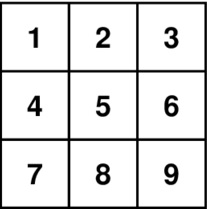
\includegraphics{images/grid.jpg}
    \caption{Példa a szomszédos cellákra}
    Az 1-es cella szomszádja a 2-es, 3-as, 4-es, 7-es cella.
    \label{fig:cella-pelda}
\end{figure}
\begin{figure}
\centering
\begin{minipage}{.5\textwidth}
  \centering
  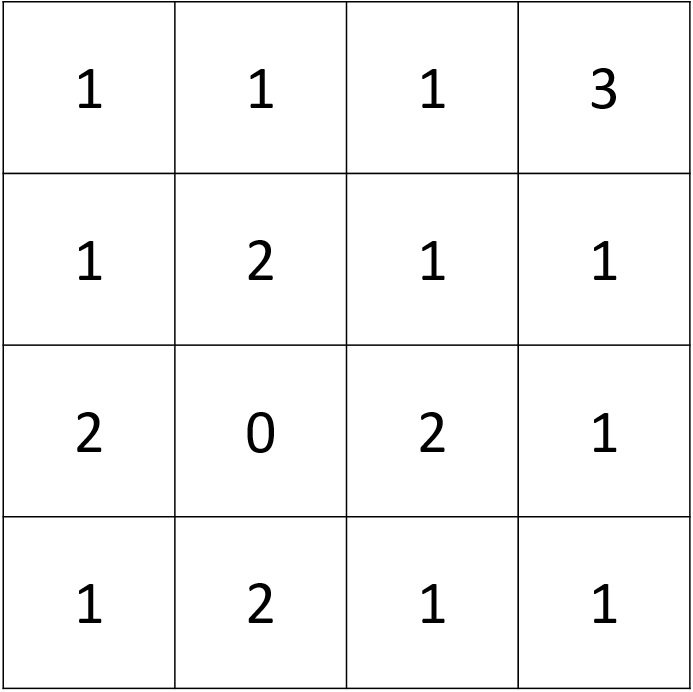
\includegraphics[width=190pt]{images/reference-table.jpg}
  \caption*{Kiinduló tábla}
\end{minipage}%
\begin{minipage}{.5\textwidth}
  \centering
  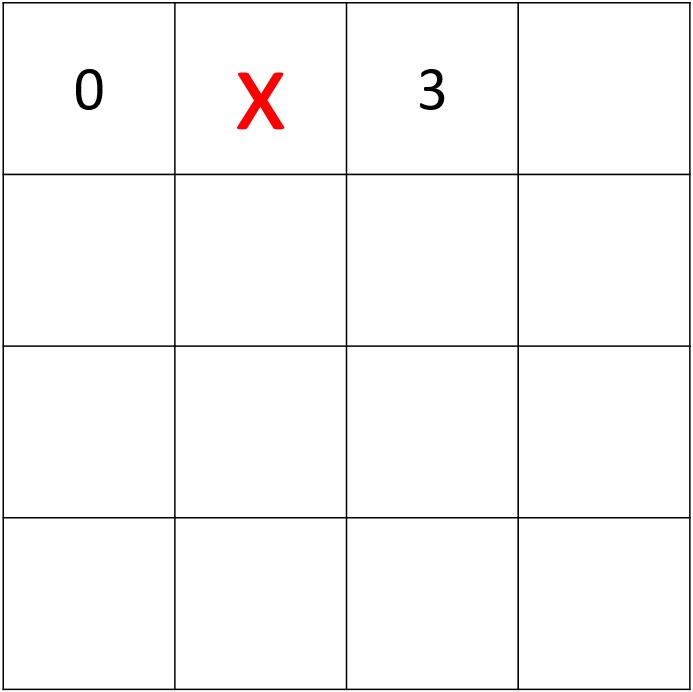
\includegraphics[width=190pt]{images/Invalid.jpg}
  \caption*{Elakadás az outputon}
\end{minipage}
\caption{Példa elakadási helyzetre}
  A hármas cella mellé csak egyes cella, a nullás cella mellé csak kettes cella kerülhet, így a kettő között nem lehet semmilyen cella.
\label{fig:elakadas}
\end{figure}

\newpage

\subsection{Implementáció}
Az implementációhoz először választanunk kell egy képet. Válasszunk egy egyszerű, pár különálló blokkból álló képet például a képen láthatót. Ha nem jól elválasztható blokkokból áll a kép, akkor az algoritmusunkat nem tudjuk használni.
 \begin{figure}[h]
     \centering
     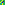
\includegraphics[width=80pt]{images/block-easy.png}
     \caption{Egyszerű input kép}
     \label{fig:egyszeru-kep}
 \end{figure}
Látható, hogy a kép 4 elkülöníthető blokkból áll, zöld, sárga, kék, piros blokkokból. Gondoljunk ezekre a blokkokra, úgy mintha virágok lennének egy mezőn. A zöld blokkok jelölik a füvet, a színesek pedig a virágokat. Az elvárásunk az lehet, hogy egy nagyobb mezőt alkossunk, és a virágok aránya nagyjából megegyező legyen az input képben látható arányokkal.\\
A következő lépésben feldaraboljuk ezt a képet, és kialakítjuk a cellákat. A feldarabolt cellákat szeretnénk megtekinteni és tetszőlegesen paraméterezni. Ehhez használjuk a Unity egyik felxibilis eszközét, a ScriptableObject-et.
Ebben az osztályban tároljuk le a cellának a képét, a súlyát és a szomszédjait. Ebből az objektumból annyit kell automatikusan létrehoznia a beolvasónknak, ahány cellára daraboltuk fel az inputot. Miután megtötént a létrehozás, feltöltjük az objektumokat.
 \begin{figure}[h]
\centering
\begin{minipage}{.5\textwidth}
  \centering
  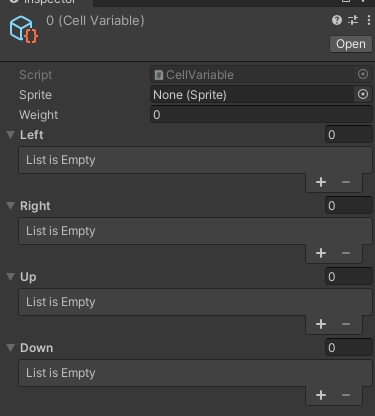
\includegraphics[width=0.99\textwidth]{images/scriptable-object-cell.jpg}
  \caption{Üres ScriptableObject}
  \label{fig:ures-scriptable}
\end{minipage}%
\begin{minipage}{.5\textwidth}
  \centering
  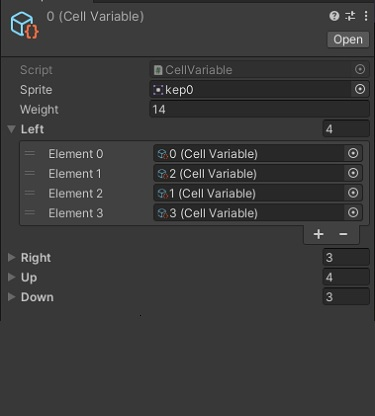
\includegraphics[width=0.99\textwidth]{images/scriptable-object-cell-toltott.jpg}
  \caption{Feltöltött ScriptableObject}
  \label{fig:teli-scriptable}
\end{minipage}
\caption*{Cella-paraméter leíró objektumok}
\end{figure}

A feltöltött objektumokat pedig megadjuk az algoritmusnak, ezekből lesznek a cellák.
\newpage
Az algoritmus futása előtt kiválasztjuk a preferált módszert a \ref{item:modszer}-es lépésben definiáltak közül, illetve hogy mekkora outputot szeretnénk generálni.\\
A példához egy $25X25$ nagyságú outputot választottam. A véletlenszerű generálás nem adott eredményt, mert csak elakadást produkált.
 \begin{figure}[h]
\centering
\begin{minipage}{.5\textwidth}
  \centering
  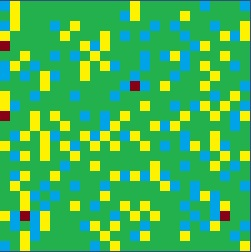
\includegraphics[width=0.99\textwidth]{images/horizontal.jpg}
  \caption{Horizontális generálás}
  \label{fig:wfc-horizontal}
\end{minipage}%
\begin{minipage}{.5\textwidth}
  \centering
  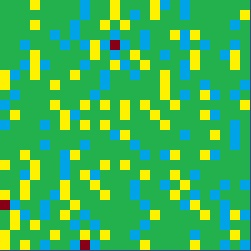
\includegraphics[width=0.99\textwidth]{images/vertical.jpg}
  \caption{Vertikális generálás}
  \label{fig:wfc-vertical}
\end{minipage}
\begin{minipage}{.5\textwidth}
  \centering
  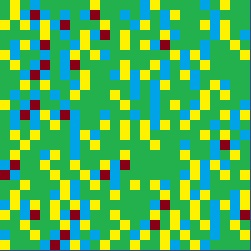
\includegraphics[width=0.99\textwidth]{images/entropy.jpg}
  \caption{Entrópiás generálás}
  \label{fig:wfc-entropy}
\end{minipage}
\caption*{Output generálás különböző módszerekkel}
\end{figure}